\section{Edit Quality}
\label{sec:editquality}

The problem with measuring text contribution quality alone is that it
measures only one kind of user behavior: inserting and deleting of text.
Another important behavior of users is to rearrange text
(possibly with minor edits) so that it improves the flow or
readability of the text.
In traditional publishing, this is a function provided by the
editor --- and both content creation and editing for grammar and
style are valuable to the quality of the final product.
Is there any notion equivalent to text survival for edits?
In struggling to answer this question, we first had to measure
the size of an ``edit contribution,'' which naturally led us to the
\intro{edit distance}~\cite{Levenshtein1966,Tichy1984,Cormode2007,Adler2007}
measure.

\subsection{Edit Distances}
\label{sec:eq-distances}

Edit distance~\cite{Levenshtein1966} is typically used as a way to
measure how many insertions, deletions, and replacements are needed to
transform one string into another (the collection of these operations
is called an \textit{edit script}), and is thus defined as the sum of the
number of those operations (that is, the size of the edit script).
Other formulations exist for edit distance, and within the
context of the WikiTrust project, we were already computing
text differences as part of our author tracking algorithms,
so we chose to define the distance between two revisions
in terms of the edit script generated by our greedy text
matching algorithm from Chapter~\ref{ch:diff}.
The elements making up the edit script generated by WikiTrust are:
\begin{itemize}
\item $\mathbf{Move}(i_1, i_2, k)$ -- a block of text of
    length $k$ words which matches between the source string
    and target string.\footnote{In WikiTrust, we index our hashtable
    of word positions by word pairs, so that a match will always
    be of length~2 or greater.}
    The match starts at position $i_1$ in the source string,
    and starts at position $i_2$ in the target string.
\item $\mathbf{Delete}(i, k)$ -- the text starting at position $i$
    and extending for length $k$ words was deleted from the source string.
\item $\mathbf{Insert}(i, k)$ -- the text starting at position $i$
    and extending for length $k$ words was inserted into the target string.
\end{itemize}

If we let $E(m,n)$ be the edit script set of elements describing the
transformation from the source string \words{\version{m}}
to the target string \words{\version{n}},
then we can define terms for the total amount of insertions,
deletions by summing over all the matching elements:
\begin{align*}
  I_{tot}(m,n) =& \sum_{\mathbf{Insert}(i, k) \in E(m,n)} k \\
  D_{tot}(m,n) =& \sum_{\mathbf{Delete}(i, k) \in E(m,n)} k \\
\end{align*}
%
We must take more care in quantifying how much \textit{movement}
was involved in an edit; simply summing the size of each
\textbf{Move} operation is not sufficient, because our edit script
includes \textit{all} matching text as these operations.
What we would like is to only count those blocks of text that
were actually rearranged.
Let $l_m = | \words{\version{m}} |$ and $l_n = | \words{\version{n}} |$.
Each time a block of text of length $k$ exchanges position
with a block of text of length $k'$, we count this distance
as $k \cdot k' / \max(l_m, l_n)$.
Thus, a word that moves across $k'$ other words contributes
$k / \max(l_m, l_n)$ to the distance; the contribution
approaches~1 as the word is moved across the whole document.
The total contribution from \textbf{Move} operations is
then given by:
%
\begin{align*}
  M_{tot}(m,n) =& \sum_{\substack{
        \mathbf{Move}(i_1, i_2, k) \in E(m,n) \\
        \mathbf{Move}(i'_1, i'_2, k') \in E(m,n) \\
        i_1 < i'_1 \;\And\; i_2 > i'_2
        }} \frac{k \cdot k'}{\max(l_m, l_n)} \\
\end{align*}

We then define the edit distance between revisions
\version{m} and \version{n} as
\begin{equation}
    \dist{}{m,n} = \max(I_{tot}(m,n), D_{tot}(m,n))
        + M_{tot}(m,n)
        - \frac{1}{2}\min(I_{tot}(m,n), D_{tot}(m,n)) \\
\label{eq:dist}
\end{equation}
The motivation for this formulation of edit distance is
to try to account for replacements, which appear within
the edit script as both insertion and deletions --- but the
position information required to match them is not preserved
by the difference algorithm.
By subtracting a correction term, we make the assumption
that edits with both insertions and deletions make some
replacements, which are being counted in both types of edit.

\subsection{Edit Longevity}

Given a method to measure the size of an edit contribution,
the problem still remains of how to compute whether that
contribution is preserved in future revisions.
An idea we considered is summing the edit distances of
sequential revisions, and comparing that against the edit
distance between the first and last revisions.
This has the problem that it roughly assumes that all
contributions are completely preserved or completely
reverted, but the idea of mapping out the edit distances of
multiple revisions led to another idea that we favor.

Instead of trying to measure whether an edit is preserved,
let us ask the question, ``Does this edit move us in the
direction of the future of the article or does it move us away
from the future?''
This suggests consideration of three versions: the one being
evaluated, one in its past, and one in its future.
Figure~\ref{fig-editcontr} visually represents two cases in
evaluating revision \version{k}, using \version{k-1}
and \version{j} (where $j > k$) as guide posts for the general
path that the evolution of the article is taking.
If a contribution moves us in the general direction of
the future but has some extraneous text that is deleted,
we get the case shown in Figure~\ref{fig-editcontr-a}:
the distance \dist{}{k,j} is smaller than the distance \dist{}{k-1,j}.
If the edits of \version{k} do not contribute at all to the
future of the article, then we have the case shown in
Figure~\ref{fig-editcontr-b}:
the distance \dist{}{k,j} is larger than the distance \dist{}{k-1,j}.

\begin{figure}[t]
\centering
\subfigure[Graphical representation of a good edit contribution.]{
\label{fig-editcontr-a} 
\framebox{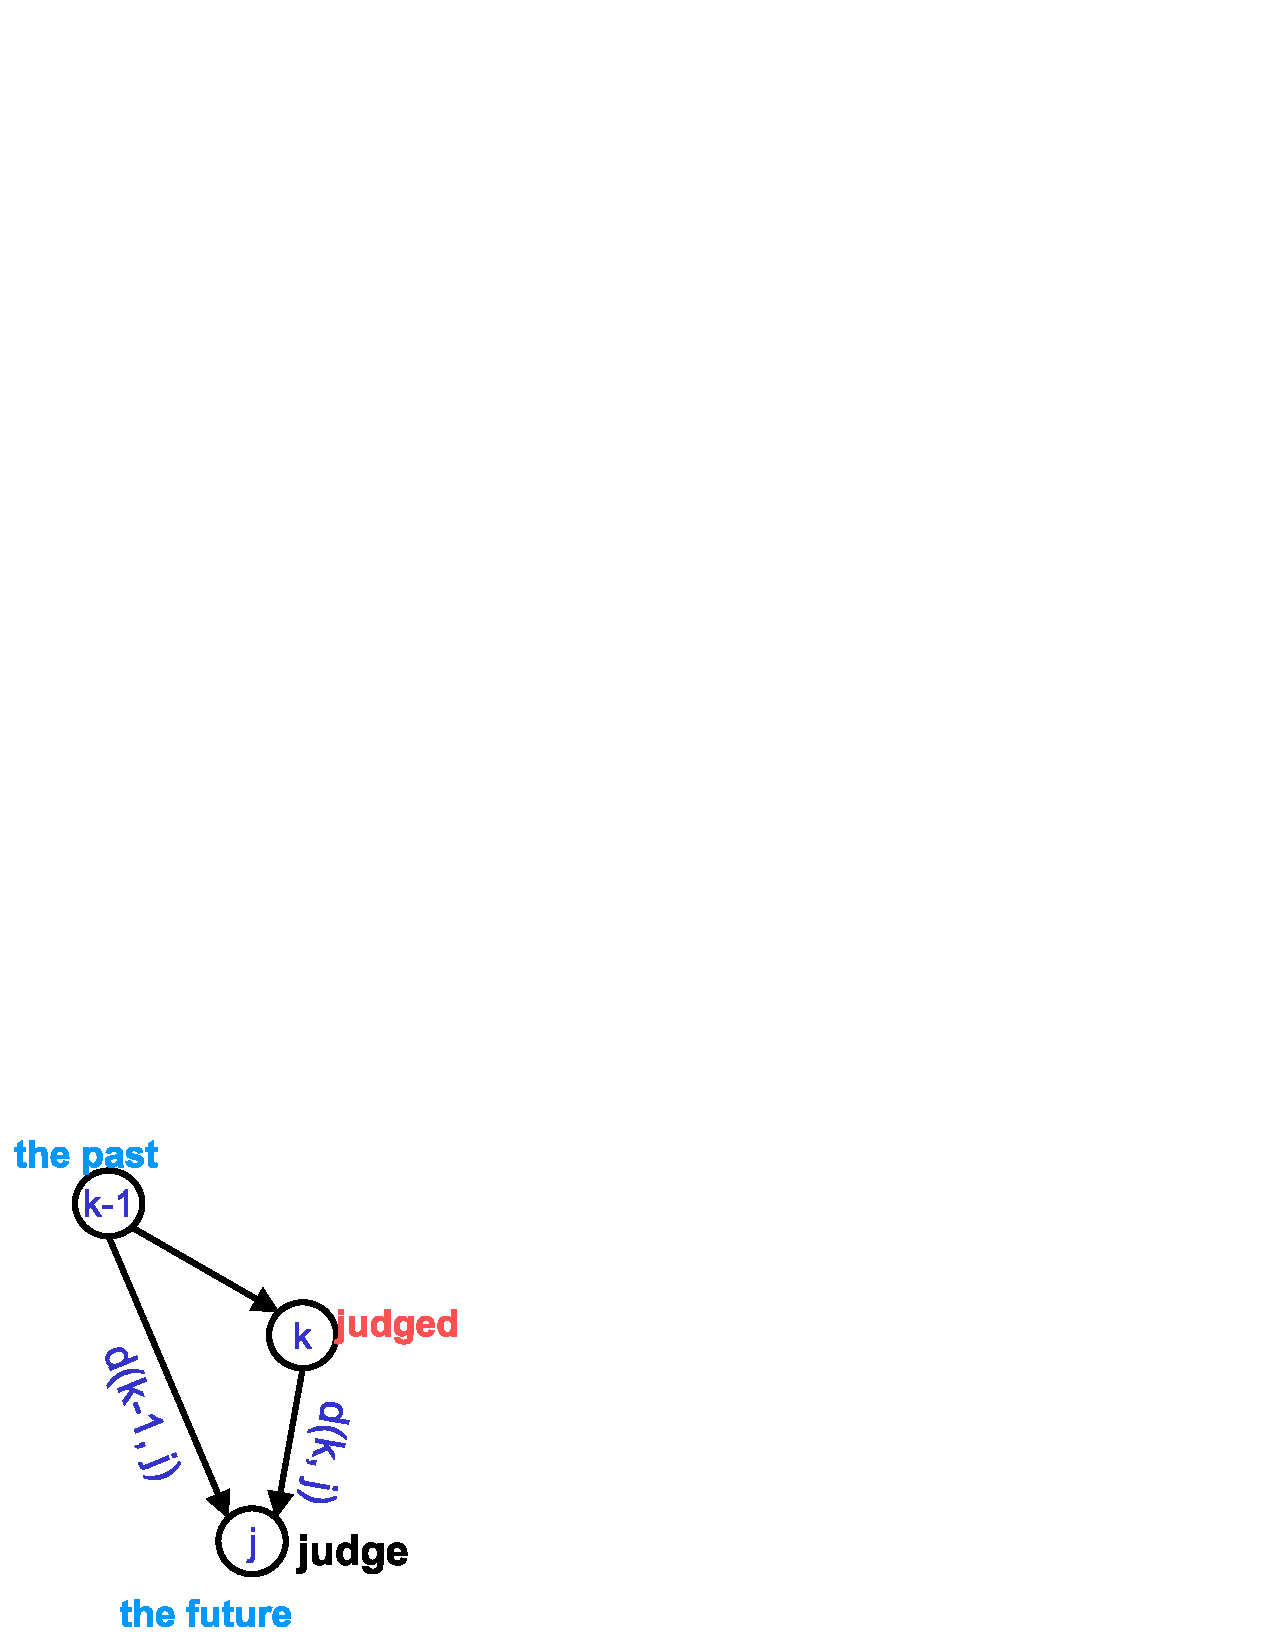
\includegraphics[width=0.35\textwidth]{part-F70-editquality/editcontr-good}}
}
\hspace{1ex}
\subfigure[Graphical representation of a bad edit contribution.]{
\label{fig-editcontr-b}
\framebox{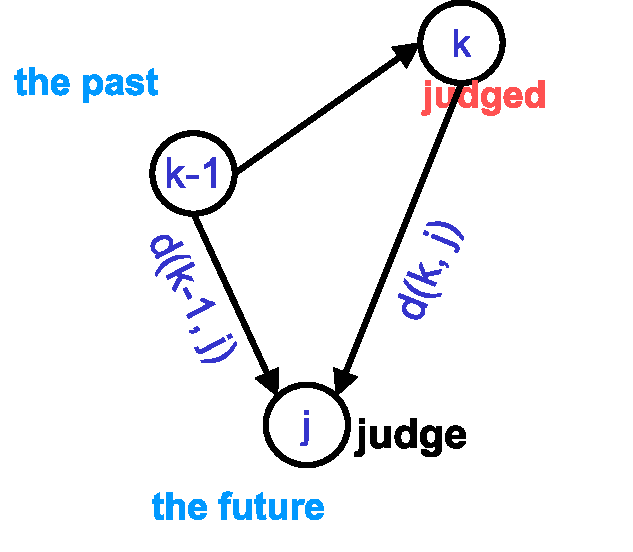
\includegraphics[width=0.40\textwidth]{part-F70-editquality/editcontr-bad}}
}
\caption{To measure the quality of version \version{k}, we also
	look at the previous version \version{k-1} and some future
	version \version{j}.
	The three versions form a triangle, using
	edit distance~\cite{Levenshtein1966} to define the separation
	between each other.
	Intuitively, we know that when \version{k} is good,
	the distance to the future, $\dist{}{k, j}$,
	will be shorter than if \version{k} is bad.
	(When \version{k} is bad, more editing is required to
	bring it back to a better version, plus the editing
	to bring it to the future.)
}
\label{fig-editcontr}
\end{figure}

So now we have a very simple analysis of comparing
\dist{}{k,j} with \dist{}{k-1,j} to tell us whether the
quality of revision \version{k} is \textit{good} or \textit{bad}
(at least with respect to \version{k-1} and \version{j}).
We would like to have more gradation in a quality measure than
just the two extremes; we would like to know \textit{how} good
or bad an edit is.
To answer this question, we thought that a good measure would
be to compare the total work done by \revauthor{\version{k}},
with the amount of progress made towards the future.
That is, if an author writes a 600~word essay about a topic,
but only 20~words are actually kept in the article, then the
original 600~word contribution must have been pretty bad.
Instead, if 300~words remain in the article (half of them),
then the contribution could be said to be so-so.

%\begin{wrapfigure}{r}{0.55\textwidth}
\begin{figure}
\centering
\framebox{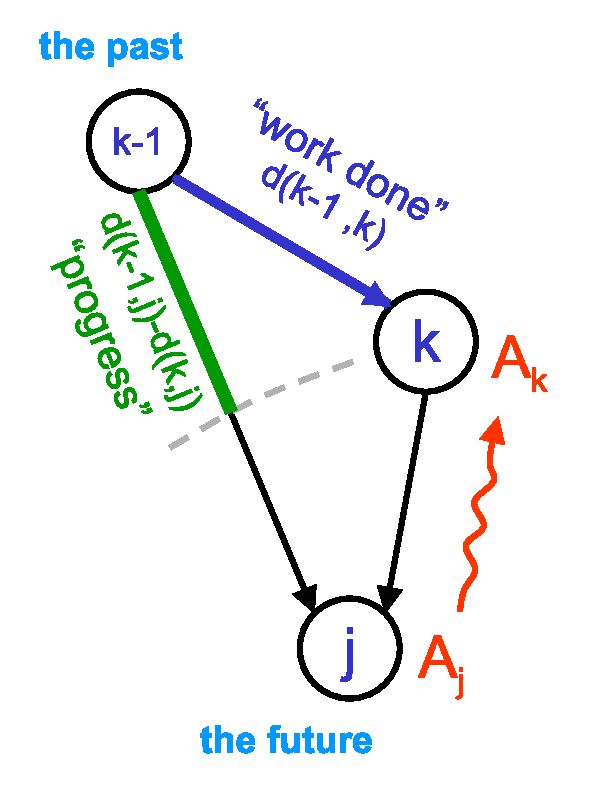
\includegraphics[width=0.35\textwidth]{part-F70-editquality/edit-longevity}}
\caption{Quality is measured by calculating how much \textit{progress}
	is made towards the future version of the article,
	and dividing that by the amount of \textit{work done}
	during the edit.}
\label{fig-editlong}
\end{figure}
%\end{wrapfigure}

We propose that a good way to measure this judgement
by \revauthor{\version{j}} of \revauthor{\version{k}},
which we call \intro{edit longevity}, is:
\begin{equation}
\esurv{}{k,k-1,j} = \frac{\dist{}{k-1,j} - \dist{}{k,j}}
                        {\dist{}{k-1,k}},
\label{eq:esurv}
\end{equation}
It compares the ``useful progress''
$\dist{}{k-1,j} - \dist{}{k,j}$
with the ``total work''
$\dist{}{k-1,k}$.
Figure~\ref{fig-editlong} presents the graphical interpretation
of the quantities involved.
  For reverted edits, the ratio \esurv{}{k,k-1,j}
  is $-1$, since all the work
  goes into \textit{increasing} the distance between \version{k} and \version{j}.
  For preserved edits, \esurv{}{k,j} is close to~1.

Note that here and in our original work on
this topic~\cite{Adler2007}, the reference revision from the past is always
the revision immediately before the revision being evaluated.
In practice, the revision immediately before might be vandalized,
so that the path from \version{k-1} to \version{j} does not
actually represent the overall trajectory of edits for the
article.
Another work dealing with
the robustness of reputation~\cite{Chatterjee2008} addresses this
shortfall.
Also, it is sometimes the case that a revision is created with
no changes (or with changes only in whitespace), so that we
have $\dist{}{k-1,k} = 0$; in this case, we ignore the triangle
and do not compute a longevity score for revision \version{k}.

\subsubsection{The Reverse Triangle Inequality}

The insight leading to Equation~\ref{eq:esurv} is that the edit distance
measure induces a topological space that relates every revision to
every other revision.
Using that model for our intuition, we can describe the evolution of
an article from its creation to the most recent revision as a trajectory
in the space.
This is very much like a drunken walk across a bridge;
there is a clear start and a clear end, but an inebriated
pedestrian won't follow a straight line.
Using the straight line between start and end as a reference,
we can measure the pedestrian's forward progress, as well as
how much wasted effort he puts into moving sideways along the bridge.
Figure~\ref{fig-editlong} is applying that analogy in our
edit distance based topology, and shows one way to measure
the forward progress.
(Another way to measure the progress would be to compute the
angles of the triangle and multiply the sine of the
work done angle by its length.)

Continuing with physical intuition of how revisions can be
related to each other, the reverse triangle
inequality~\cite{wiki:TriangleInequality} allows us to put bounds
on the value of Equation~\ref{eq:esurv}.
The reverse triangle inequality states that any side of
a triangle is greater than the absolute value of the difference
of the other two sides:
\begin{equation}
| \dist{}{k-1,j} - \dist{}{k,j} | \le \dist{}{k-1,k}
\end{equation}
The two sides of this equation are exactly the two terms
of our fraction, so that we can conclude that edit longevity
varies from $-1$ to $+1$.

There is just one problem with this analysis: it depends on
the triangle inequality holding.
Unfortunately, this is not actually the case; we adjust for
this by limiting the result to the range $-1$ to $+1$,
with any value beyond that range being capped to the closest
value within the range.
\mynote{For additional discussion of the triangle inequality issue,
see Appendix~\ref{app:editlong-data}.}

\subsection{Edit Longevity Quality}

Our strategy for turning edit longevity into a quality measure
is to compute an average of edit longevity from several different
perspectives.
Edit longevity requires two landmarks to base a judgement on:
some revision in the past, and some revision in the future of
the version being judged.
For simplicity, we choose the revision immediate previous to
the one being evaluated as the landmark in the past.
That is, if we are evaluating \version{k}, then we choose
\version{k-1} as one of the reference points.
Our motivation for choosing only a single previous revision
as a reference point is that past revisions cannot be making
any implicit statements about a revision that has not happened
yet.\footnote{In hindsight, the previous revision might have been
blanked or otherwise vandalized, so that multiple previous revisions
should actually be considered.}

Our central idea for extracting community sentiment from the
revision history of an article is to examine what happens to an
author's contribution as the article continues to evolve.
We say that later versions of the article act as \intro{judges}
of the contribution, because each later author implicitly makes
the decision to delete or revise existing text in the article.
For text quality we used the ten following revisions as judges,
but this allows the possibility for the author being judged
to act as his own judge.
We address this gap in the case of turning edit longevity into
a quality by defining a map
\begin{equation*}
J : \articles \times \versions{} \times \mathbb{Z} \to 2^\versions{}
\end{equation*}
which, for an article $a \in \articles$,
returns the set of up-to $n$ versions that act as judges
to version $\version{k} \in \versions{a}$, with the proviso
that author of \version{i} does not act as his own judge:
\begin{equation}
\judges{a}{n}{k} = \{ j : \exists j \in \mathbb{Z}\ .\ 0 < j - k \le n
    \wedge \revauthor{\version{k}} \ne \revauthor{\version{j}} \}
\label{def:judges}
\end{equation}

With our reference points for the past and future selected, we
can define the average edit longevity as follows:
\begin{equation}
\quality{elong}{a,n}{k} = \frac{1}{|\judges{a}{n}{k}|} \cdot
      \sum_{i \in \judges{a}{n}{k}} \esurv{}{k,k-1,i}
\label{def:elong}
\end{equation}

